\chapter{Introduction}
\vspace{-1.4em}
The introduction orients the reader to your thesis. It should present the nature and scope of the problem in terms of applications to `real world' problems (what motivates the study); refer briefly to associated and relevant literature already published; state the method of investigation (the main technical issues, including important limitations in scope); and describe the report that follows (a sort of road-map, so that the reader knows what's to come).This is well shown in \cite{Xu_2007}.\\

\begin{figure}[ht] 
    %[ht] tells latex to place the figure in its relative position after the body of text. without this flag, it will default to floating/placed at the bottom of page despite the content that is after it.
 \begin{center}
%trim option's parameter order: left bottom right top, remove square brackets for no trim
 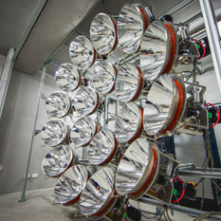
\includegraphics[width=0.5\textwidth]{images/antenna_array}
 \end{center} 
 \caption{Example figure.}
 \label{fig:antenna_array}
\end{figure}

